\documentclass[tikz,convert={density=150,size=600,outext=.png}]{standalone}
\usetikzlibrary{shapes, calc, arrows, fit, positioning, decorations, patterns, decorations.pathreplacing, chains, snakes}

\begin{document}
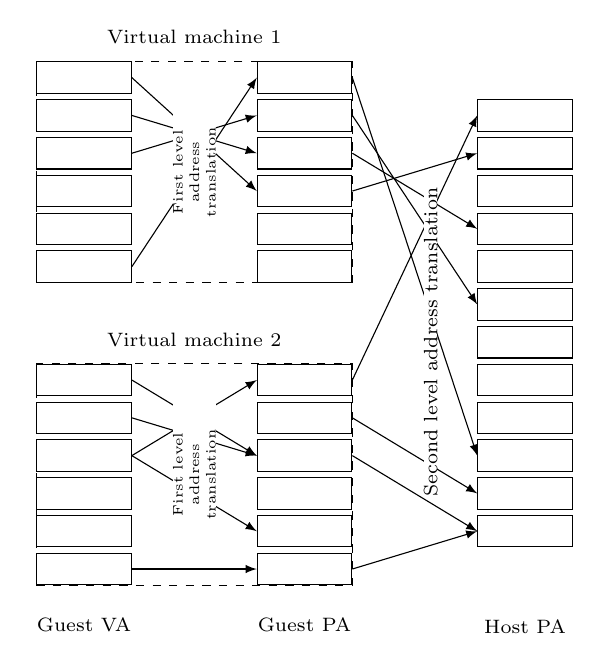
\begin{tikzpicture}[>=latex, font=\scriptsize, scale=0.8]
  \foreach \x in {0,1}
  {\foreach \y in {0,1,2,3,4,5,8,9,10,11,12,13} { % vertical offsets of two groups
          \node[draw, minimum width=1.2cm, minimum height=0.4cm, inner sep=0pt] at (\x*3.5cm, -\y * 0.6 cm) (vpage-\x-\y) {};
    };
  };

  \foreach \y in {0,1,2,3,4,5,6,7,8,9,10,11} {
          \node[draw, minimum width=1.2cm, minimum height=0.4cm, inner sep=0pt] at (7cm, -0.6cm -\y * 0.6 cm) (ppage-\y) {};
  };

  \node[draw, dashed, inner sep=0pt, fit=(vpage-0-0) (vpage-1-5) ]  (vm1-border) {} ;
  \node[draw, dashed,  inner sep=0pt, fit=(vpage-0-8) (vpage-1-13) ]  (vm2-border) {} ;
  \node[fill=white, inner sep=1pt, yshift=0.3cm] at (vm1-border.north) {Virtual machine 1};
  \node[fill=white, inner sep=1pt, yshift=0.3cm] at (vm2-border.north) {Virtual machine 2};

  \node[below=.3cm of vpage-0-13, align=flush left] {Guest VA};
  \node[below=.3cm of vpage-1-13, align=flush left] {Guest PA};
  \node[below=.8cm of ppage-11, align=flush left] {Host PA};

  \draw[->] (vpage-0-0.east) -- (vpage-1-3.west);
  \draw[->] (vpage-0-1.east) -- (vpage-1-2.west);
  \draw[->] (vpage-0-2.east) -- (vpage-1-1.west);
  \draw[->] (vpage-0-5.east) -- (vpage-1-0.west);
  \node[fill=white, rotate=90, text width=2cm, inner sep=0pt, align=center,
    font=\tiny] at (1.75, -2.5*0.6) {First level\\address translation};

  \draw[->] (vpage-0-10.east) -- (vpage-1-8.west);
  \draw[->] (vpage-0-8.east) -- (vpage-1-10.west);
  \draw[->] (vpage-0-9.east) -- (vpage-1-10.west);
  \draw[->] (vpage-0-10.east) -- (vpage-1-12.west);
  \draw[->] (vpage-0-13.east) -- (vpage-1-13.west);
  \node[fill=white, rotate=90, text width=2cm, inner sep=0pt, align=center,
    font=\tiny] at (1.75, -10.5*0.6) {First level\\address translation};

  \draw[->] (vpage-1-0.east) -- (ppage-9.west);
  \draw[->] (vpage-1-1.east) -- (ppage-5.west);
  \draw[->] (vpage-1-2.east) -- (ppage-3.west);
  \draw[->] (vpage-1-3.east) -- (ppage-1.west);

  \draw[->] (vpage-1-8.east) -- (ppage-0.west);
  \draw[->] (vpage-1-9.east) -- (ppage-10.west);
  \draw[->] (vpage-1-10.east) -- (ppage-11.west);
  \draw[->] (vpage-1-13.east) -- (ppage-11.west);
  \node[fill=white, rotate=90, inner sep=0pt] at (5.5, -7*0.6) {Second level address translation};
\end{tikzpicture}
\end{document}
